\documentclass{article}
\usepackage[utf8]{inputenc}
\usepackage{graphicx}
\graphicspath{ {./imagenes/} }
\usepackage{multicol}
\usepackage[spanish, english]{babel}
\usepackage[left=3cm,right=3cm,top=3cm,bottom=3cm]{geometry}

\providecommand{\keywords}[1]{
  \small	
  \textbf{\textit{\quad \quad Keywords: }} #1}

\providecommand{\pclave}[1]{
  \small	
  \textbf{\textit{\quad \quad Palabras Clave: }} #1}

%Idiomas: \selectlanguage{english} \selectlanguage{spanish}

\begin{document}

\title{Trabajo Encargado N°2: Principios de Diseño y DDD}

\begin{titlepage}
\begin{figure}[htb]
\begin{center}

\includegraphics[width=5cm]{logo.png}
\end{center}
\end{figure}
\vspace*{-0.25in}
\begin{center}
\large{UNIVERSIDAD PRIVADA DE TACNA}\\
\vspace*{-0.025in}
INGENIERÍA DE SISTEMAS  \\

\vspace*{0.5in}
\begin{large}
TITULO:\\
\end{large}

\vspace*{0.1in}
\begin{Large}
\textbf{Principios de Diseño y DDD} \\
\end{Large}

\vspace*{0.3in}
\begin{Large}
\textbf{CURSO:} \\
\end{Large}

\vspace*{0.1in}
\begin{large}
CALIDAD Y PRUEBAS DE SOFTWARE\\
\end{large}

\vspace*{0.3in}
\begin{Large}
\textbf{DOCENTE:} \\
\end{Large}

\vspace*{0.1in}
\begin{large}
 Ing. Patrick Cuadros Quiroga\\
\end{large}

\vspace*{0.2in}
\vspace*{0.1in}
\begin{large}

Integrantes: \\
\begin{flushleft}
Sivirichi Falcón, Ricardo Alonso\hfill(2018060905) \\
Chambilla Maquera, Araceli Noemi\hfill(2018060897)\\
Arenas Paz Soldan, Miguel Jesus\hfill(2017059282)\\
Cotrado Marino, Ana Luz\hfill(2018060907)\\

\end{flushleft}
\end{large}

\vspace*{0.1in}
\begin{large}
Tacna - Perú\\
2020
\end{large}
\end{center}
\end{titlepage}

\selectlanguage{spanish}
\begin{abstract}
\quad En este artículo abordaremos sobre los principios DRY, principios SOLID y  DDD para comprender la forma en que se pueda implementar en los diseños de software en el día a día. La metodología usada fue el análisis y síntesis de la información de diversos libros y artículos, con la finalidad de demostrar un concepto claro sobre una base fundamental de un buen desarrollo. Este artículo concluye que los principios de diseño son muy útiles como una guía de comportamiento amplia aplicable a muchas situaciones.

\end{abstract}
\pclave{Principios de Diseño, Principios SOLID, Principios DRY, diseño dirigido por el dominio.}

\selectlanguage{english}
\begin{abstract}
\quad In this article we will cover the DRY principles, SOLID principles and DDD to understand how it can be implemented in software designs on a day-to-day basis. The methodology used was the analysis and synthesis of information from various books and articles, in order to demonstrate a clear concept on a fundamental basis of good development. This article concludes that critics accuse them of being ambiguous, confusing, complicating the code, delaying the development process, and even label them as totally wrong and unnecessary. 

\end{abstract}
\keywords{Design Principles, SOLID Principles, DRY Principles, domain-driven design.}

\begin{center}\rule{1\textwidth}{0.05mm} \end{center}

\selectlanguage{spanish}

\begin{multicols}{2}
\section{Introducción}
 \quad Las tecnologías están en constante expansión y evolución, diseñando nuevas técnicas para cumplir con su fin. En el desarrollo de software, las herramientas y pautas para la elaboración de productos software constituyen una pieza en constante evolución, necesarias para la toma de decisiones sobre los proyectos a realizar. 
 
 Uno de los arquetipos para el desarrollo de software es el denominado Domain Driven Design, donde es importante conocer ampliamente el negocio que se desea modelar en forma de dominio, a través de ciertos elementos como la identificación de entidades o un lenguaje cuidado.
 
 La gran evolución de la computación en la nube y los servicios con funciones específicas, denominados microservicios, introducen ciertas necesidades en los algoritmos computacionales que manejan, como la seguridad en el procesamiento de los datos. Para alcanzar estos requisitos evitando mecanismos de control costosos, la programación funcional provee de múltiples elementos que confieren al lenguaje de capacidades para alcanzar este fin, como inmutabilidad de los datos.

\section{Desarrollo}
 \quad Un principio se puede entender como una guía de comportamiento amplia aplicable a muchas situaciones. En general un principio no te dice que hacer exactamente, sino que te da pistas de cuál es la acción correcta a través de una gran cantidad de situaciones, pero los detalles están a cargo de ti mismo.

Hablando de principios de diseño de software, puedes pensar en ellos como en un faro que te guía a través de la oscuridad de los requerimientos del problema. A diferencia de los patrones de diseño, no establecen los pasos necesarios para aplicarlos, ni siquiera la situaciones en las que son aplicables, de hecho, se pueden crear varios patrones y reglas basándonos en ellos.

\subsection{Principios DRY}
 \quad En diseño orientado a objetos, El principio No te repitas (en inglés Don't Repeat Yourself o DRY, también conocido como Una vez y sólo una) es una filosofía de definición de procesos que promueve la reducción de la duplicación especialmente en programación. 

DRY implica que, cualquier funcionalidad existente en un programa debe existir de forma única en él, o lo que es lo mismo, no debemos tener bloques de código repetidos (Álvarez Caules, 2012). 

(Hunt and Thomas, 2000), puntualizan que la única manera de desarrollar software confiablemente y hacer desarrollos más fáciles de entender y mantener, es seguir lo que llaman el principio DRY: “cada pieza de conocimiento debe tener una representación sencilla, individual, autoritativa dentro de un sistema”.

Según este principio toda pieza de información nunca debería ser duplicada debido a que la duplicación incrementa la dificultad en los cambios y evolución posterior, puede perjudicar la claridad y crear un espacio para posibles inconsistencias.

Por "pieza de información" podemos entender, en un sentido amplio, desde datos almacenados en una base de datos pasando por el código fuente de un programa de software hasta llegar a información textual o documentación.

\subsection{Principios SOLID}
SOLID es el acrónimo para un conjunto de prácticas que, cuando se implementan juntos, hacen que el código sea adaptable al cambio. Las practicas SOLID fueron introducidas por Bob Martin hace casi 15 años. Aun así, estas prácticas no son tan ampliamente conocidas como podría ser y quizás debería serlo (McLean Hall, 
2014). \\ SOLID nos facilita a los desarrolladores escribir software fácil de mantener y extender. En resumen, es aplicar los principios SOLID de manera adecuada nos permite tener código limpio, que se traduce en sistemas más flexibles y estables.
\begin{center}
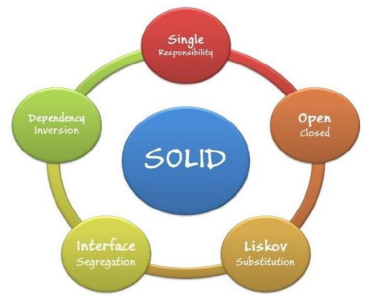
\includegraphics[width=6cm]{imagenes/principiosSOLID.png}

La Figura N° 2.3, muestra los cinco principios que conforman SOLID.
\end{center}

\begin{enumerate}
\item SRP. El Principio de Responsabilidad Única. Una clase debe tener una, sólo una, razón para cambiar.
\item OCP. El Principio Abierto/Cerrado. Debe ser capaz de extender un comportamiento de clases, sin modificarlo.
\item LSP. El Principio de Sustitución de Liskov. Las clases derivadas deben ser sustituibles por sus clases base.
\item ISP. El Principio de Segregación de Interfaces. Hacer interfaces de grano fino que son específicos del cliente.
\item DIP. El Principio de Inversión de Dependencia. Depende de abstracciones, no de concreciones.
\end{enumerate}

\subsection{Domain driven design}
DDD o diseño dirigido por el dominio es tanto una manera de pensar como un conjunto de prioridades, con el objeto de acelerar el desarrollo de proyectos de software que deben lidiar con dominios complicados.

Al desarrollar software basado en modelos se debe tener cierto grado de habilidad para entender cómo funciona un modelo en la vida real. Conocer el funcionamiento del dominio y ser capaz de abstraer las características principales del mismo en un modelo es lo que se conoce como DDD.

Para trabajar con DDD es necesario definir un conjunto de conceptos que conforman un dominio dentro del marco de este modelo de desarrollo de software:
\begin{itemize}
    \item Bounded Context, de forma individualizada, es un módulo que forma el sistema y define al más alto nivel de granularidad una funcionalidad completa.
    \item Elementos del domino, esto son los objetos que el dominio utiliza para trabajar. Entre ellos hay que destacar tres elementos principales.
    \begin{itemize}
        \item Entidad, elemento que se caracteriza por ser identificable por un único valor o un conjunto de estos.
        \item Objeto de valor, elemento similar a la entidad, salvo que es identificable por el conjunto completo de su contenido y, en caso de modificar cualquier valor del mismo, se obtendría otro elemento distinto.
        \item Servicio, elemento de más alto nivel que, normalmente, modela un caso de uso del negocio en cuestión, y trabaja conjuntamente con entidades y objetos de valor.
    \end{itemize}
    \item Elementos de gestión del ciclo de vida, mediante los que se puede mantener la duración de entidades y de objetos de valor en el sistema a través de múltiples patrones. De ellos destacan:
    \begin{itemize}
        \item Factorías, las cuales permiten mantener en una misma localización la creación de entidades similares, siendo este un servicio de creación y, si es posible, inicialización de instancias.
        \item Agregados, que permiten definir y acotar consistentemente la lógica que las entidades u objetos de valor pueden tomar. De esta forma un agregado puede manejar la consistencia sobre la cantidad de elementos disponibles para su compra o controlar las fechas de creación y cierre.
        \item Repositorios, que se emplean para persistir y conservar entidades, objetos de valor o agregados cuando estos ya no son necesarios para el estado del negocio, pero si puedan serlo en un estado futuro.
    \end{itemize}
    \item Lenguaje ubicuo, con el que se puede definir un lenguaje adecuado y acotado al negocio a abstraer en el sistema. Con este lenguaje se intenta definir interfaces expresivas de modo que un programador pueda entender el negocio sin necesidad de conocer la implementación de la API, lo que se conoce como un DSL.
\end{itemize}

\section{Conclusiones}
 Los principios SOLID es algo básico que te ayudará en tu día a día. Si desarrollas software con un diseño de alta calidad te permitirá construir software mantenible, escalable y reutilizable. Cuando desarrollas cualquier software, hay dos conceptos muy importantes: cohesión (cuando dos partes distintas de un sistema trabajan juntas para tener mejor resultado que ambas partes trabajando de manera individual) y acoplamiento (puede verse como un grado de dependencia en una clase, método o otra entidad de software).

\section{Recomendaciones}
Se recomienda el uso de los principios S.O.L.I.D. en el refactoring y/o
desarrollo de aplicaciones en Java, con la finalidad de obtener aplicaciones con una adecuada calidad interna y que sean fáciles de adaptar a los cambios y exigencias del negocio.

Asimismo, una propuesta de diseño como DDD puede no ser totalmente compatible con las herramientas y tecnologías elegidas para el desarrollo de un proyecto. Si se quieren mantener en el mismo, resulta necesario resolver las inconsistencias o contradicciones que puedan surgir.
\end{multicols}

\begin{thebibliography}{XXX0000}
    \bibitem{LLA2019} Llanos Zela, G. R. (2019). Las mejores prácticas para los programadores aplicando unit test y code coverage (Doctoral dissertation).

    \bibitem{JAR2019} Jaraba Romero, H. (2019). Desarrollo de un sistema software para la gestión de las operaciones de una central nuclear (Doctoral dissertation).

    \bibitem{SUC2018} Sucasaca Surco, W. (2018). Uso de los principios DRY y SOLID en un proceso de refactoring de una aplicación web java para mejorar su calidad interna.

    \bibitem{CUE2011} Cuesta-Arvizu, H., and Ruiz-Castilla, J. (2011). Patrones de Diseño para el Modelado Orientado a Dominio aplicando el Paradigma Orientado a Objetos. Comité Editorial, 2(2), 18.

    \bibitem{GAM2003} Gamma, E., Helm, R., Johnson, R., and Vlissides, J. (2003). Patrones de Diseño, Elementos de software orientado a objetos reutilizable. Pearson Educación.
    
    \bibitem{SHV2021} Shvets, A. (2021). Dive into Design Patterns: Vol. 1.7 (v2021 ed.) [Libro electrónico]. \\https://refactoring.guru/es/design-patterns/book
\end{thebibliography}

\end{document}
